\chapter{Speech Processing}\label{ch:speech_processing}

Speech is an effortless and highly efficient form of communication. Continuous speech recognition software is readily available from local computing stores and comes complete with microphone, allowing the user to dictate text directly into a document. The current technology is not perfect but is getting better \cite[p.~396]{callan2003artificial}.\\

Words are carried as sound waves, which are analog signals. In order for the speech to be processed, it needs to be run through a signal processor that selects the frequencies and amplitude of the signal. Further on, the signal is mapped to individual sound units called phones. These phones need to be identified and grouped in such a way to ensure that each word has a different phonetic structure, otherwise, words would be impossible to distinguish from one another. \\

\begin{table}[]
\centering
\caption{Phones}
\label{my-label}
\begin{tabular}{ll}
{[}ay{]} & iris \\
{[}b{]}  & bin  \\
{[}er{]} & bird \\
{[}l{]}  & lip  \\
{[}p{]}  & pin  \\
{[}th{]} & thin
\end{tabular}
\end{table}

Phones can have different sounds depending on context. For example, the phone th in the word \textit{three} has a different sound to th in \textit{then}. To overcome these different variations of the same phones, it is better to abstract the phones into a generalized grouping called a \textbf{phoneme}. Phonemes are written in-between forward slashes (\textit{/th/}) and they will have a specific pronunciation for each sound, depending on the context. These phonemes are used as a transitional layer when trying to convert speech to text and vice versa when speech needs to be synthesized.\\

\section{Signal processing}

Sound waves that carry human speech are variations in air pressure. The key components of a sound wave are its \textbf{amplitude}, which measure the intensity of the sound and the \textbf{frequency}, which describes the rate at which the amplitude varies over time. When speaking in a microphone, the change in air pressure causes the diaphragm to oscillate. The size of the oscillations is directly proportional to the amplitude of the signal, while the rate at which the diaphragm oscillates gives represents the rate at which the air pressure changes. At specific time intervals, the signal can be sampled and the data can be used in a wide array of digital signal processing tools. For example, the digital signal can be plotted as an x-y plot, where the y-axis defines the amplitude and the x-axis shows the passage of time. The frequency can be easily be determined from the plot as we find the number of cycles that the signal does per second.\\

Although a visual difference can be seen when plotting vowels and consonants, a visual inspection of the waveform will not reveal any critical information, making it impossible to see all the phonemes.\\

\subsubsection{ Fourier transform}

To analyse a discrete signal we use the Fourier transform. This allows us to convert the signal in the frequency domain and deconstruct it in a series of simple sine waves. These sine waves have specific amplitudes and frequencies and while plotting the FFT of the signal, the dominant waves can be identified by the intensity of the amplitude.\\

In Figure \ref{fig:FFT}, a visual representation of the FFT is shown and it can be seen that there are a lot of frequencies that make up the word "hello". The dominant ones are in the range of 500Hz, and considering that this recording has a minimum amount of noise in it we have to consider the full range of the frequencies, from zero and up to 3500Hz.

\begin{figure}
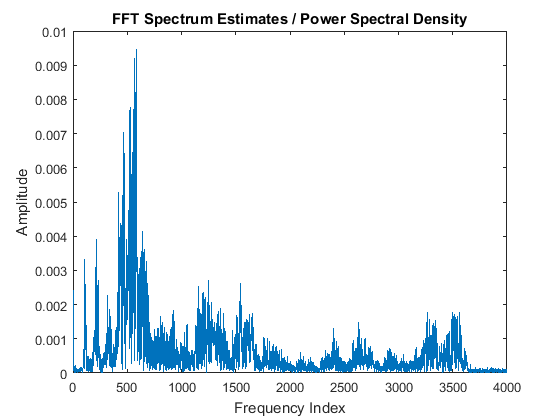
\includegraphics[scale=1]{FFTpicture2}
\centering
\caption{Example of the FFT function computed for the word "Hello"}
\label{fig:FFT}
\end{figure}
